\part[Projektdokumentation]{Projektdokumentation
                  \begin{center}
                     \begin{minipage}[c]{10.7cm}
                      \small Hitobito: Neue Generation von Personen-Filtern \\
                      Autor: Marc Egli
                     \end{minipage}
                  \end{center}
                 }
\chapter{Einführung}
Puzzle ITC ist ein schweizer Anbieter für Softwarelösungen. Die Firma hat ihren Hauptsitz in Bern,
besitzt aber weitere Standorte in Zürich, Luzern und Deutschland (Thüringen). Puzzle bietet als Unternehmen
die ganze Palette an IT-Services an, von Digital Transformation bis hin zu Data Analytics. Nebst den vielen Angeboten
tritt Puzzle dabei immer seine Grundwerte nach aussen, welche im Puzzlehouse abgebildet werden.

\begin{figure}[h]
   \centering
   
\includegraphics[width=1\textwidth,]{puzzle-house.png}
   \caption{Rollen in Scrum}
\end{figure}

Hitobito ist eines der Angebote von Puzzle. Es ist ein Community-Management Tool und
als Open-Source Projekt auf Github zu finden. Das Tool wird von zahlreichen Verbänden, Parteien
und Organisationen verwendet und befindet sich darum in einer kontinuerilichen Weiterentwicklung. Mit dem Wagons-Gem
ermöglicht es Hitobito zudem spezielle Kundenanpassungen in einem eigenen "Wagon" zu vollziehen, ohne die Software anderer
Kunden mit-anzupassen.

Ich selbst arbeite jetzt seit einem halben Jahr im Hitobito und nahm darin vor allem Upgrades und Migrationen vor. So durfte ich
bspw. das Upgrade von RoR (Ruby on Rails) von 6.1 auf 7.1 vornehmen oder die Migration von MySQL auf Postgres vollziehen.

Da Hitobito von zahlreichen Kunden verwendet wird, ist die Applikation über die Jahre gewachsen. Viele Features wurden implementiert,
um sie schnell dem Kunden zur Verfügung zu stellen. Mit einem immer wachsenden Anforderungskatalog ergaben sich dadurch komplexe Arbeitsabläufe
welche im Tool etabliert wurden. Einer dieser komplexen Abläufe ist die Filterung nach Personen oder Abonnemente.

Mit dieser IPA soll die Filterung zwischen diesen zwei Entitäten homogenisiert werden. Um dies zu tun,
sollen zuerst zwei bis drei Konzepte ausgearbeitet und anschliessend in einem Variantenentscheid evaluiert werden. Für die Lösungsvariante wird in einem weiteren Schritt ein PoC (Proove of Concept) implementiert. 

Nach der IPA soll basierend auf der neuen Filterlogik ein neues UI entworfen werden, um nebst der Ordnung im Backend
eine besser User Experience für den Benutzer zu schaffen.

In einer Zeit in welcher Unternehmen mehr den je Wert auf ein sauberes Design und der User Experience von Webseiten und Applikationen geben, das auch
in einer älteren Applikation zu etablieren. Gerade bei einem Community-Management Tool wie Hitobito, welches tagtäglich von 
Personen bedient werden, welche nicht das technische Know-How dahinter besitzen, ist es wichtig Arbeitsabläufe so einfach wie möglich zu entwerfen, um 
maximale Effizienz für diese Personen zu garantieren. Durch eine Vereinfachung der Hitobito-Fitler machen wir damit einen ersten Schritt in die richtige
Richtung.

\chapter{Analyse}
In der Analyse der IPA wird der Rahmen geschaffen in welchem man später während des Implementierens arbeitet. 
Sie befasst sich mit der Aufnahme von Ist- und Zielzustand und definierte Funktionale sowie nicht funktionale Anforderungen.
Es wird definiert wo sich die IPA abgrenzt. 

\section{Ist-Zustand}

\subsection{Personenlisten}
Aktuell kann ein Nutzer über den Button Neuer-Filter auf die Filter Seite navigieren. 
\begin{figure}[h]
   \centering
   \fbox{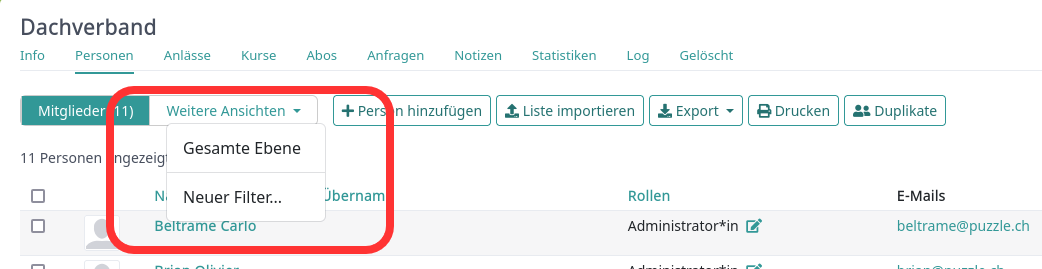
\includegraphics[width=1\textwidth,]{hitobito_header.drawio.png}}
   \caption{Hitobito Personenlisten Filtererstellung}
\end{figure}

\newpage 

Auf dieser definiert er die Filterungskriterien für die Attribute Rollen, Qualifikationen,
Felder, Sprache und Tags. 
\begin{figure}[h]
   \centering
   \fbox{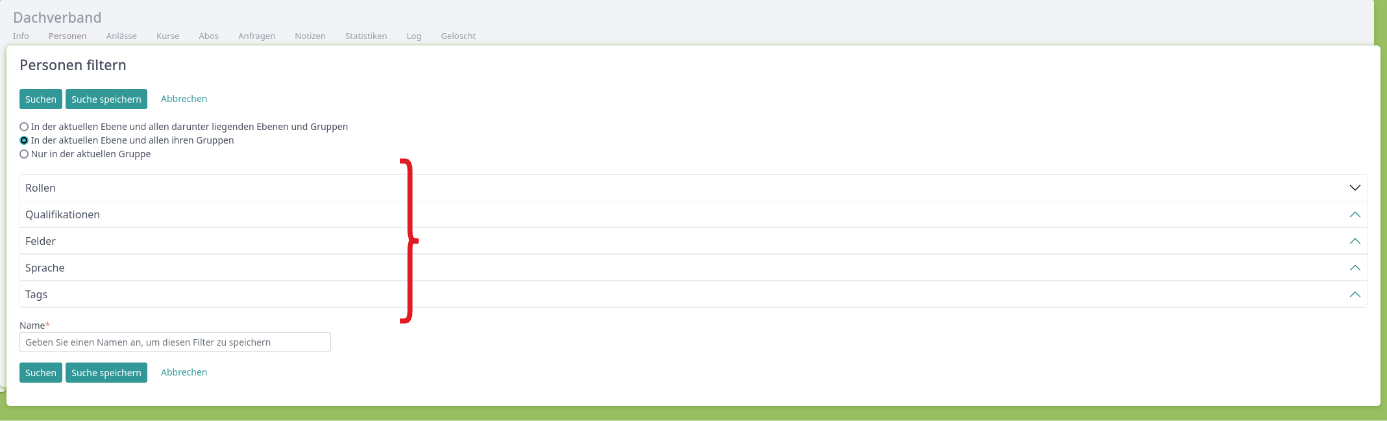
\includegraphics[width=1\textwidth,]{hitobito_person_list_filter.drawio.png}}
   \caption{Hitobito Personenlisten Filterkriterien}
\end{figure}

Anschliessend ist es dem Nutzer möglich seinen Filter über einen Button für die Wiederverwendung
zu speichern.
\begin{figure}[h]
   \centering
   \fbox{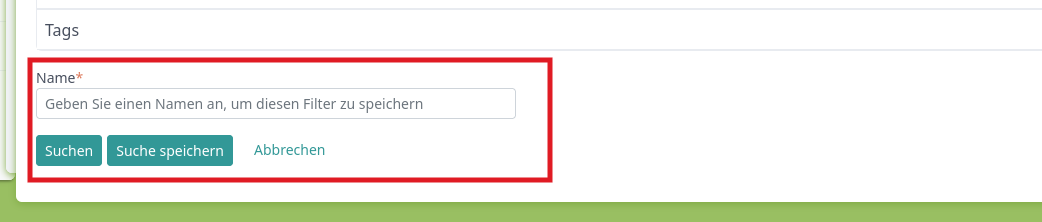
\includegraphics[width=1\textwidth,]{save_filter.drawio.png}}
   \caption{Hitobito Personenlistenfilter Speicherung}
\end{figure}

\newpage

Technisch sind die Personenlisten-Filter nach folgendem Sequenzdiagramm aufgebaut:
\begin{figure}[h]
   \centering
   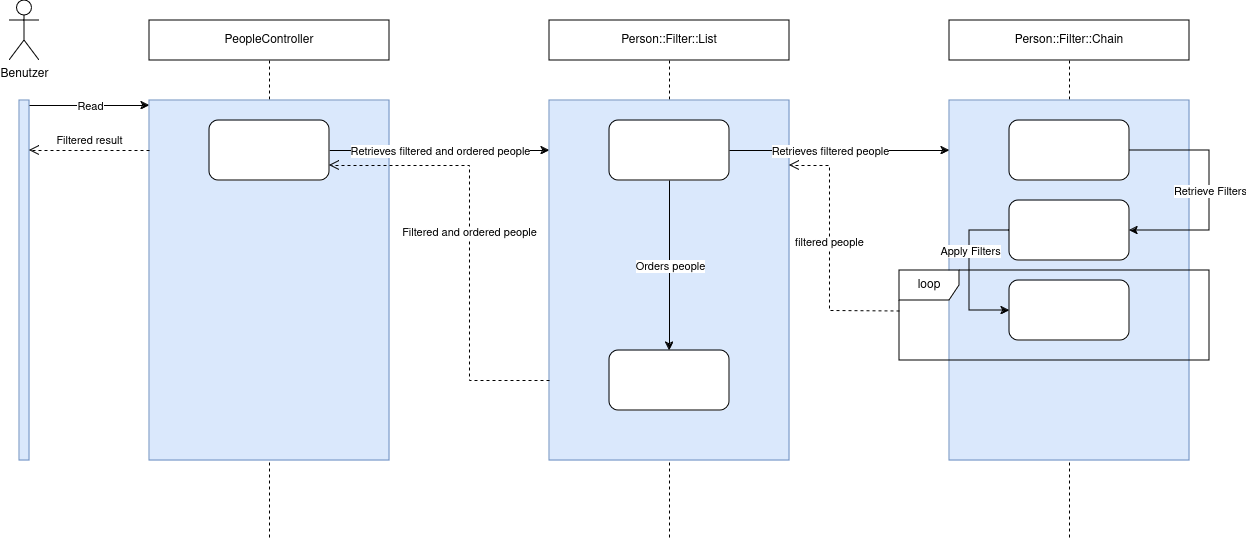
\includegraphics[width=1\textwidth,]{person_filter.png}
   \caption{Sequenzdiagramm Personenlisten Filter}
\end{figure}

\begin{table}[h!]
   \begin{tabular}{|L{0.4\textwidth}|L{0.5\textwidth}|}
       \hline
       \rowcolor{puzzleblue} \multicolumn{2}{|l|}{\color{white}\textbf{Beschreibung Sequenzdiagramm}} \\[12pt]
       \hline
       PeopleController & Der PeopleController nimmt den Request des Benutzers entgegen und erwidert die gefilterten und sortierten Personen auf welche der Benutzer zugreifen darf. \\
       \hline
       Person::Filter::List & Personen auf welche der Benutzer keinen Zugriff hat werden rausgefiltert und anschliessend sortiert. \\
       \hline
       Person::Filter::Chain & Definiert anhand der Request Parameter vom Controller die Filter und wendet diese in einem Loop via chain-pattern an. \\
       \hline
     \end{tabular}
     \caption{Beschreibung Sequenzdiagramm}
\end{table}

\newpage

\subsection{Abonnemente}
Auf den Abonnementen kann der Nutzer Filterkriterien in den globalen Bedingungen definieren.

\begin{figure}[h]
   \centering
   \fbox{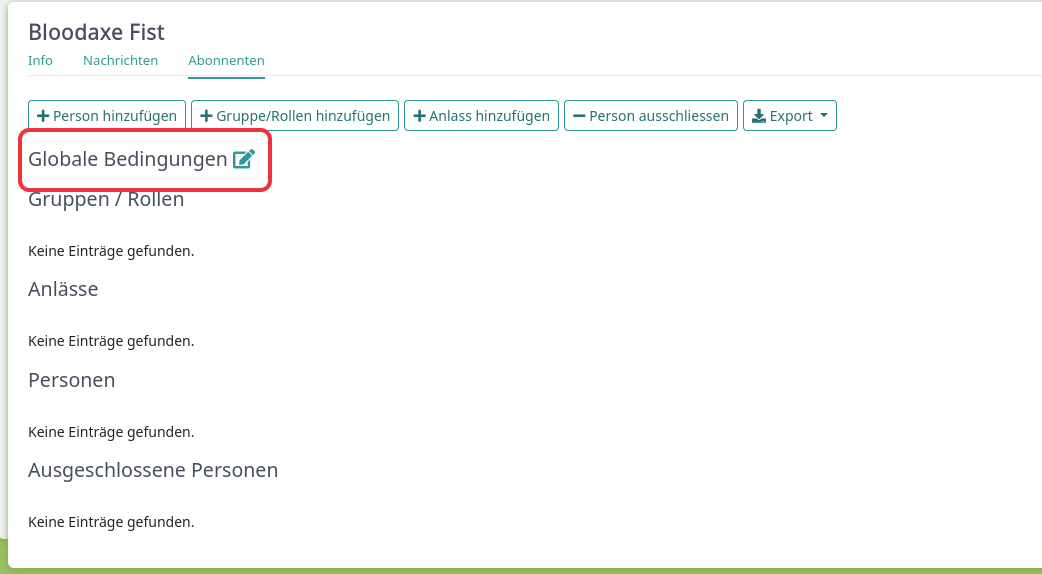
\includegraphics[width=1\textwidth,]{hitobito_global_conditions.drawio.png}}
   \caption{Hitobito Globale Bedingungen}
\end{figure}

Unter diesen kann der Nutzer per Dropdown entscheiden für welche Attribute er die Filterkriterien definieren möchte.
Er kann auch bereits gesetzte Kriterien entfernen. Pro Filterkriterium entscheidet er im weiteren, mit welcher Genauigkeit
nach diesem Filterkriterium gesucht wird. Bei Zahlen ist es möglich die Genauigkeiten ist genau, ist höher als und ist kleiner als 
einzustellen. Bei Textvergleichen sind es ist genau, enthält, enthält nicht.
\begin{figure}[h]
   \centering
   \fbox{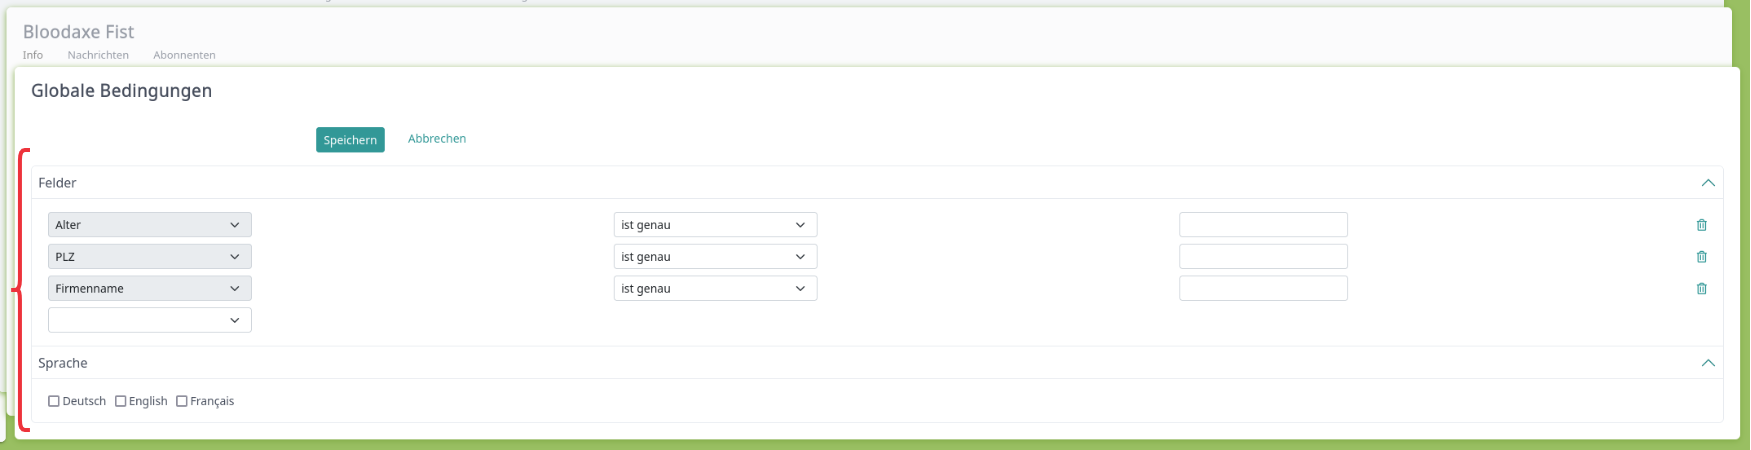
\includegraphics[width=1\textwidth,]{hitobito_filter_conditions.drawio.png}}
   \caption{Hitobito Filterkriterien}
\end{figure}

\newpage

Hat der Nutzer seine Filterkriterien und die dazugehörigen Genauigkeiten definiert, kann er sie über den
Speicher-Button persistieren. Im Anschluss werden die ausgewählten Filterkriterien in den Globalen Bedingungen angezeigt
und ein Success-Alert ausgelöst der die Aktualisierung bestätigt.
\begin{figure}[h]
   \centering
   \fbox{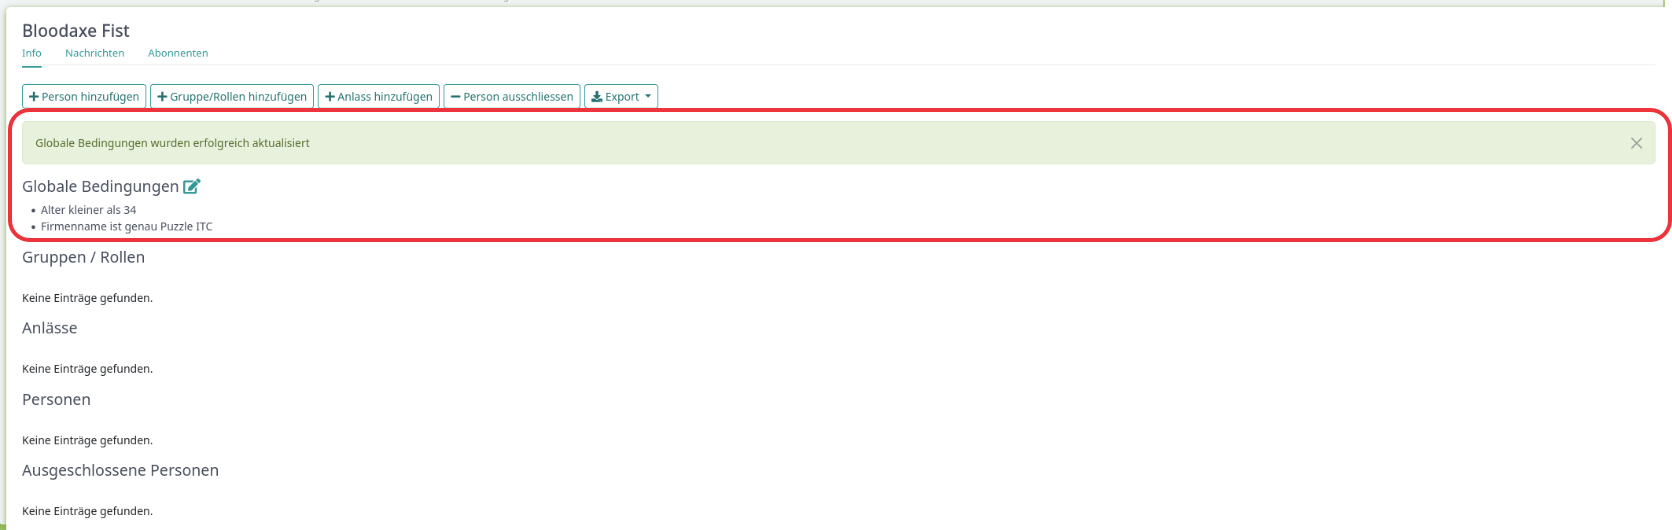
\includegraphics[width=1\textwidth,]{hitobito_filter_created.drawio.png}}
   \caption{Hitobito Filterkriterien}
\end{figure}

Technisch haben sind die Abonnemente nach folgendem ERD aufgebaut.
\begin{figure}[h]
   \centering
   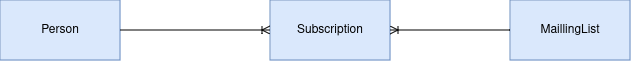
\includegraphics[width=1\textwidth,]{subscriptions_erd.drawio.png}
   \caption{Hitobito Subscription ERD}
\end{figure}

Es ist zu beachten: Eine Person kann mehrere Subscriptions besitzen und jede Subscriptions ist einer
Mailling list zugerodnet. Somit muss bei der Filterung nach Subscriptions zuerst die MaillingList included
werden, damit man auf dieser danach die Filterung ausführen kann.

\newpage

Die Globalen Filterungskriterien für die Abonnemente werden in dem Modell der MaillingList
abgespeichert. Dadurch ergibt sich folgendes Sequenzdiagramm.
\begin{figure}[h]
   \centering
   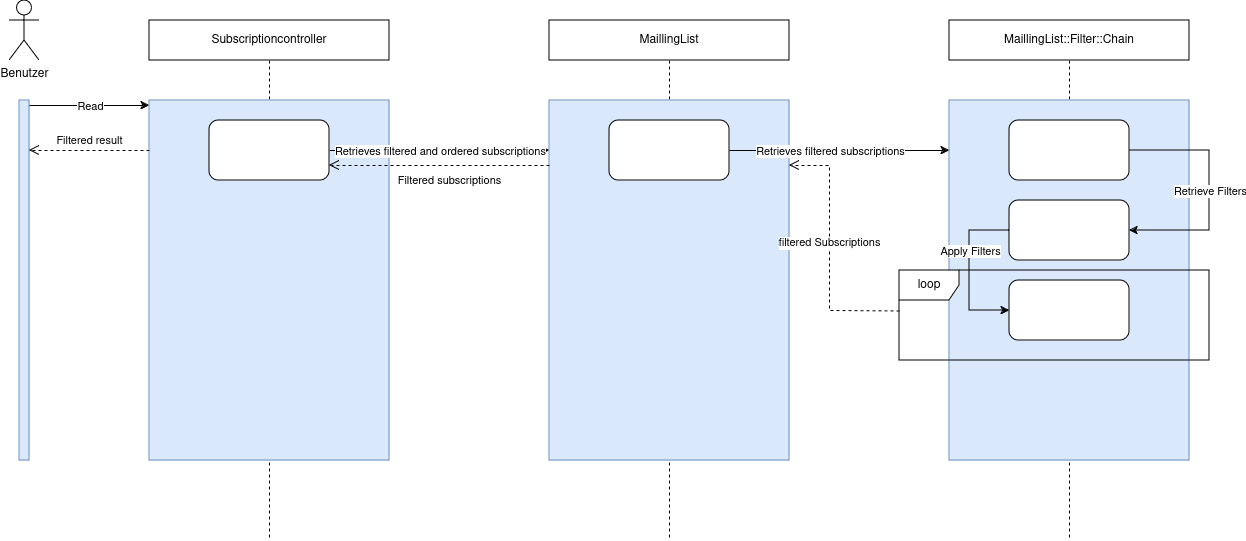
\includegraphics[width=1\textwidth,]{subscriptions_filter.drawio.png}
   \caption{Hitobito Abonnementen Sequenzdiagramm}
\end{figure}

\begin{table}[h!]
   \begin{tabular}{|L{0.4\textwidth}|L{0.5\textwidth}|}
       \hline
       \rowcolor{puzzleblue} \multicolumn{2}{|l|}{\color{white}\textbf{Beschreibung Sequenzdiagramm}} \\[12pt]
       \hline
       SubscriptionController & Der SubscriptionController nimmt den Request des Benutzers entgegen und erwidert die gefilterten und sortierten Personen auf welche der Benutzer zugreifen darf. \\
       \hline
       MaillingList & Fetcht Subscriptions aus der Datenbank und macht Aufruf zum MaillingList::Filter::Chain \\
       \hline
       MaillingList::Filter::Chain & Holt die Filterkriterien aus der Datenbank und filtered die Subscriptions danach aus. \\
       \hline
     \end{tabular}
     \caption{Beschreibung Sequenzdiagramm}
\end{table}

\section{Soll-Zustand}
Das neue Konzept für die Abonnementen- und Personenlistenfilterung soll durch den gleichen Prozess laufen. 
Die beiden Filterungsprozesse sollen dabei zu einem homogenisiert werden und trotzdem die gleichen Funktionalitäten bieten.
Bestehende Datenmodelle sollen ebenfalls fusioniert werden.

\section{Persönliche Vorgehensziele}
\begin{table}[h!]
   \begin{tabular}{|L{0.4\textwidth}|L{0.5\textwidth}|}
       \hline
       \rowcolor{puzzleblue} \multicolumn{2}{|l|}{\color{white}\textbf{Zeitrahmen}} \\[12pt]
       \hline
        Beschreibung & Der erstellte Zeitplan, Meilensteine und Sprints werden erfolgreich eingehalten. \\
       \hline
       Messbarkeit & Die IPA wird komplett und in der definierten Frist abgeben. \\
       \hline
     \end{tabular}
     \caption{Zeitrahmen}
\end{table}

\begin{table}[h!]
   \begin{tabular}{|L{0.4\textwidth}|L{0.5\textwidth}|}
       \hline
       \rowcolor{puzzleblue} \multicolumn{2}{|l|}{\color{white}\textbf{Filterprozesse}} \\[12pt]
       \hline
       Beschreibung & Die Verständnis der Hitobito Filterlogik wird vertieft. \\
       \hline
       Messbarkeit & Zukünftig dient Kandidate als Anlaufstelle für Fragen zur Filterung und
       kann dieses Wissen in anderen Aufträgen anwenden. \\
       \hline
     \end{tabular}
     \caption{Filterprozesse}
\end{table}

\begin{table}[h!]
   \begin{tabular}{|L{0.4\textwidth}|L{0.5\textwidth}|}
       \hline
       \rowcolor{puzzleblue} \multicolumn{2}{|l|}{\color{white}\textbf{Ruby on Rails}} \\[12pt]
       \hline
       Beschreibung & Das Wissen rund um das Ruby on Rails Framework und Aufbau von Domain und Modellklassen 
       wird vertieft. \\
       \hline
       Messbarkeit & Erlangtes Wissen kann in zukünftiger Entwicklung an Features eingesetzt werden. \\
       \hline
     \end{tabular}
     \caption{Ruby on Rails}
\end{table}

\begin{table}[h!]
   \begin{tabular}{|L{0.4\textwidth}|L{0.5\textwidth}|}
       \hline
       \rowcolor{puzzleblue} \multicolumn{2}{|l|}{\color{white}\textbf{Konzeption}} \\[12pt]
       \hline
       Beschreibung & Der Kandidat ist in der Lage Features oder Umstrukturierungen an einer Applikation
       selbständig zu konzipieren. \\
       \hline
       Messbarkeit & Konzept für neues Filterverhalten wurde sauber aufgestell und Entscheidung dafür begründet.  \\
       \hline
     \end{tabular}
     \caption{Konzeption}
\end{table}

\section{Anforderungen}
\subsection{Nicht funktionale Anforderungen}

\begin{table}[h!]
   \begin{tabular}{|L{0.3\textwidth}|L{0.6\textwidth}|}
       \hline
       \rowcolor{puzzleblue} \multicolumn{2}{|l|}{\color{white}\textbf{Erweiterbarkeit, NfA. 1}} \\[4pt]
       \hline
       Beschreibung & Bei der Implementation der neuen Filterlogik wird beachtet, dass zukünftig weitere
       Filterkriterien oder Genauigkeiten vom Kunden gewünscht werden können. \\
       \hline
       Messbarkeit & Die Implementation wurde nachhaltig umgesetzt und bietet Möglichkeiten zur Erweiterung.  \\
       \hline
     \end{tabular}
     \caption{Erweiterbarkeit}
\end{table}

\begin{table}[h!]
   \begin{tabular}{|L{0.3\textwidth}|L{0.6\textwidth}|}
       \hline
       \rowcolor{puzzleblue} \multicolumn{2}{|l|}{\color{white}\textbf{Performance, NfA. 2}} \\[4pt]
       \hline
       Beschreibung & Die Implementation des neuen Filterungskonzeptes soll die gleiche
       Leistungsfähigkeit wie die jetztige Implementation vorweisen. \\
       \hline
       Messbarkeit & Ladezeit der Personenlisten und Abonnemente bleibt gleich.  \\
       \hline
     \end{tabular}
     \caption{Performance}
\end{table}

\begin{table}[h!]
   \begin{tabular}{|L{0.3\textwidth}|L{0.6\textwidth}|}
       \hline
       \rowcolor{puzzleblue} \multicolumn{2}{|l|}{\color{white}\textbf{Security, NfA. 3}} \\[4pt]
       \hline
       Beschreibung & Filterungen sollen auf dem Datensatz gemacht werden, welche durch das can-can-can
       Gem verfiziert hat. \\
       \hline
       Messbarkeit & Nutzer können keine Daten einsehen, auf welche sie keine Berechtigungen haben.  \\
       \hline
     \end{tabular}
     \caption{Security}
\end{table}

\begin{table}[h!]
   \begin{tabular}{|L{0.3\textwidth}|L{0.6\textwidth}|}
       \hline
       \rowcolor{puzzleblue} \multicolumn{2}{|l|}{\color{white}\textbf{DRY, NfA. 4}} \\[4pt]
       \hline
       Beschreibung & Der Code wurde nach dem DRY (Don't Repeat Yourself) Prinzip implementiert. \\
       \hline
       Messbarkeit & Es finden sich keine doppelten Klasse oder unnötige Wrapper.  \\
       \hline
     \end{tabular}
     \caption{DRY}
\end{table}

\newpage

\begin{table}[h!]
   \begin{tabular}{|L{0.3\textwidth}|L{0.6\textwidth}|}
       \hline
       \rowcolor{puzzleblue} \multicolumn{2}{|l|}{\color{white}\textbf{Dokumentation, NfA. 5}} \\[4pt]
       \hline
       Beschreibung & Code wurde dokumentiert. \\
       \hline
       Messbarkeit & Codingfiles sind mit verständlichen Kommentaren versehen.  \\
       \hline
     \end{tabular}
     \caption{Dokumentation}
\end{table}
 
\subsection{Funktionale Anforderungen}
\begin{table}[h!]
   \begin{tabular}{|L{0.3\textwidth}|L{0.6\textwidth}|}
       \hline
       \rowcolor{puzzleblue} \multicolumn{2}{|l|}{\color{white}\textbf{Konzept, fA. 1}} \\[4pt]
       \hline
       Beschreibung & Das erstellte Konzept führt beide Filterprozesse zusammen. \\
       \hline
       Messbarkeit & Es gibt im Hitobito ein homogenisierter Fitlerprozess der für weiter Filterungen
       wiederverwendet werden kann.  \\
       \hline
     \end{tabular}
     \caption{Konzept}
\end{table}

\begin{table}[h!]
   \begin{tabular}{|L{0.3\textwidth}|L{0.6\textwidth}|}
       \hline
       \rowcolor{puzzleblue} \multicolumn{2}{|l|}{\color{white}\textbf{Filterkriterien, fA. 2}} \\[4pt]
       \hline
       Beschreibung & Alle bisherigen Filterungskriterien werden weiterhin unterstützt. \\
       \hline
       Messbarkeit & UI ist immer noch gleich bedienbar wie vor der IPA.  \\
       \hline
     \end{tabular}
     \caption{Filterkriterien, fA. 2}
\end{table}

\section{Abgrenzung}

Während der IPA wird auf einem geforkten Repository gearbeitet, sowohl im Hitobito Core-Wagen wie auch
im Generic Wagon. Jeglich Commits und Push erfolgen auf den Master Branch des geforkten Repositories. Durch diese 
Abkapselung wird sichergestellt das die Weiterentwicklung von Hitobito nicht den Erfolg dieser IPA gefährden. 
 
\chapter{Entwurf}
\section{Anwendungskonzept}
Das Anwendungskonzept beschreibt wie ein Benutzer die Funktionalität dieser Arbeit verwendet und welche Anwendungsfälle
daraus entstehen.


\subsection{Anwendungsdiagram}
Es bilden sich 4 konkrete Use-Cases:
\begin{figure}[h]
   \centering
   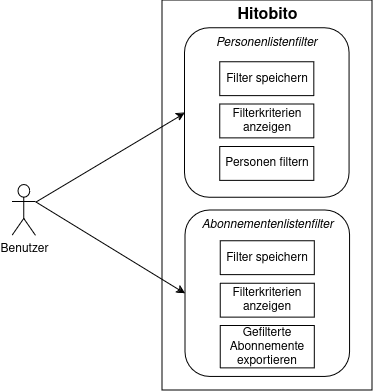
\includegraphics[width=0.85\textwidth,]{hitobito_use_case_diagram.drawio.png}
   \caption{Hitobito Filter Use Case Diagramm}
\end{figure}


\subsection{Anwendungsfälle}
Aus dem Anwendungsdiagram werden die 4 Use-Cases entnommen und hier im Detail beschrieben.

\begin{table}[h!]
   \begin{tabular}{|L{0.3\textwidth}|L{0.6\textwidth}|}
       \hline
       \rowcolor{puzzleblue} \multicolumn{2}{|l|}{\color{white}\textbf{Filter speichern}} \\[4pt]
       \hline
       Kurzbeschreibung & Der Benutzer kann die ausgewählten Fitlerkriterien speichern. \\
       \hline
       Vorbedingungen & 
       \begin{itemize}
         \item Der Benutzer besitzt die nötigen Rechte um eine Filter zu erstellen
         \item Mind. ein Filterkriterium wurde ausgewählt
       \end{itemize} \\
       \hline
       Ablauf & \begin{enumerate}
         \item Benutzer benennt den Filter, optional und nur bei Personenliste
         \item Benutzer klickt auf speichern
       \end{enumerate}  \\
       \hline
       Resultat & Der Filter wurde in der Datenbank persistiert und ein Success-Alert wird ausgegeben. \\
       \hline
   \end{tabular}
   \caption{Anwendungsfall: Filter speichern}
\end{table}

\newpage

\begin{table}[h!]
   \begin{tabular}{|L{0.3\textwidth}|L{0.6\textwidth}|}
      \hline
      \rowcolor{puzzleblue} \multicolumn{2}{|l|}{\color{white}\textbf{Filterkriterien anzeigen}} \\[4pt]
      \hline
      Kurzbeschreibung & Der Benutzer kann die Filterkriterien der gespeicherten Filter einsehen. \\
      \hline
      Vorbedingungen & 
      \begin{itemize}
         \item Der Benutzer hat einen Filter gespeichert
      \end{itemize}  \\
      \hline
      Ablauf & \begin{enumerate}
      \item Navigiert zum Filter
      \end{enumerate}  \\
      \hline
      Resultat & Die Filterkriterien werden dem Benutzer angezeigt. \\
      \hline
   \end{tabular}
   \caption{Anwendungsfall: Filterkriterien anzeigen}
\end{table}

\begin{table}[h!]
   \begin{tabular}{|L{0.3\textwidth}|L{0.6\textwidth}|}
      \hline
      \rowcolor{puzzleblue} \multicolumn{2}{|l|}{\color{white}\textbf{Personen filtern}} \\[4pt]
      \hline
      Kurzbeschreibung & Der Benutzer kann die definierten Personenlistenfilter auf eine Liste von Personen 
      anwenden. \\
      \hline
      Vorbedingungen & \begin{itemize}
         \item Benutzer besitzt Rechte um auf eine Personenliste zuzugreifen
         \item Benutzer hat einen Personenlistenfilter für diese Liste gespeichert
         \end{itemize}  \\
      \hline
      Ablauf & \begin{enumerate}
      \item Benutzer Navigiert zum Personenlistenfilter
      \item Benutzer klickt auf Filternamen
      \end{enumerate}  \\
      \hline
      Resultat & Die Personen in der Personenliste werden gefiltert und dem Benutzer angezeigt. \\
      \hline
   \end{tabular}
   \caption{Anwendungsfall: Personen filtern}
\end{table}

\begin{table}[h!]
   \begin{tabular}{|L{0.3\textwidth}|L{0.6\textwidth}|}
      \hline
      \rowcolor{puzzleblue} \multicolumn{2}{|l|}{\color{white}\textbf{Gefilterte Abonnemente exportieren}} \\[4pt]
      \hline
      Kurzbeschreibung & Der Benutzer kann die Abonnemente als PDF, CSV, Excel, etc. exportieren, dabei werden
      die gesetzten Abonnementenfilter auf diesen Export angewendet. \\
      \hline
      Vorbedingungen & \begin{itemize}
         \item Benutzer hat Rechte um Abonnemente zu bearbeiten
         \item Benutzer hat einen Abonnementenfilter gespeichert
         \end{itemize}  \\
      \hline
      Ablauf & \begin{enumerate}
      \item Benutzer zum Abonnementenfilter
      \item Benutzer wählt Zieldatei aus Dropdown aus
      \item Benutzer exportiert Abonnementenliste
      \end{enumerate}  \\
      \hline
      Resultat & Die Personen in der Personenliste werden gefiltert und dem Benutzer angezeigt. \\
      \hline
   \end{tabular}
   \caption{Anwendungsfall: Gefilterte Abonnemente exportieren}
\end{table}

\newpage
\newpage

\section{Systemkonzept}
\subsection{Betroffene Services}
\subsection{Status quo}
\subsection{Lösungsvarianten}
\subsection{Variantenentscheid}
\subsection{Ausarbeitung}

\section{Sicherheitskonzept}
\section{Fehlerbehandlungskonzept}
\section{Migrationskonzept}
\section{Testkonzept}

\chapter{Ausführung}

\section{Testprotokoll}

% Beispiel für Test Tabelle, muess je nachdem angepasst werden

\begin{table}[H]
    \rowcolors{2}{puzzleblue!25}{white}
    \begin{tabular}{|L{0.3\textwidth}|L{0.65\textwidth}|}
        \hline
        \rowcolor{puzzleblue} \multicolumn{2}{|l|}{\color{white}Resultat Testfall Nr. 1}  \\[10pt]
        \hline
        \textbf{Testname} &  \\
        \hline
        \textbf{Testkontext} &  \\
        \hline
        \textbf{Testperson} &  \\
        \hline
        \textbf{Ausführungs Datum} &  \\
        \hline
        \textbf{Testergebnis} &  \\
        \hline
        \textbf{Beschreibung} &  \\ 
        \hline
        \textbf{Fehlerklasse} & \\ 
        \hline
    \end{tabular}
    \caption{Resultat Testfall 1}
\end{table}


\chapter{Einführung}

\chapter{Sprintabschlüsse}

\section{Abschluss Sprint Initialisierung}

\section{Abschluss Sprint Umsetzung}

\section{Abschluss Sprint Finalisierung}


